\documentclass[a4paper,11pt,oneside,uplatex]{jsbook}
\usepackage{amsmath,amssymb,amsthm}
\usepackage{mathtools}
\usepackage{bm}
\usepackage[dvipdfmx]{graphicx}
\usepackage[dvipdfmx]{color}
\usepackage{ascmac}  % itembox環境
\usepackage{makeidx}
\usepackage{booktabs}
\usepackage[square,numbers]{natbib}
\usepackage{listings} % コードブロック

\theoremstyle{definition}
\newtheorem{theorem}{定理}
\newtheorem{definition}[theorem]{定義}
\renewcommand{\proofname}{\textbf{証明}}


% https://ja.overleaf.com/learn/latex/Code_listing

\definecolor{codegreen}{rgb}{0,0.6,0}
\definecolor{codegray}{rgb}{0.5,0.5,0.5}
\definecolor{codepurple}{rgb}{0.58,0,0.82}
\definecolor{backcolour}{rgb}{0.95,0.95,0.92}

\lstdefinestyle{mystyle}{
    backgroundcolor=\color{backcolour},   
    commentstyle=\color{codegreen},
    keywordstyle=\color{magenta},
    numberstyle=\tiny\color{codegray},
    stringstyle=\color{codepurple},
    basicstyle=\ttfamily\footnotesize,
    breakatwhitespace=false,         
    breaklines=true,                 
    captionpos=b,                    
    keepspaces=true,                 
    numbers=left,                    
    numbersep=5pt,                  
    showspaces=false,                
    showstringspaces=false,
    showtabs=false,                  
    tabsize=2
}

\lstset{style=mystyle}

\setlength{\textwidth}{\fullwidth}
\setlength{\textheight}{40\baselineskip}
\addtolength{\textheight}{\topskip}
\setlength{\voffset}{-0.55in}
%%
\title{{\huge 離散選択モデル入門}\\{\large Introduction to Discrete Choice Models} \\ 
$\,$\\$\,$\\$\,$\\$\,$\\$\,$\\$\,$\\$\,$\\}
\author{林~由翔\\Yuito Hayashi}
\date{2022年2月 作成 \\ 2024年4月 最終更新}
\begin{document}

\maketitle
\frontmatter
\chapter{はじめに}
この文書は、人間の選択行動を推定するときに用いられる「離散選択モデル」と、離散選択モデルの
中で代表的なモデルである「多項ロジットモデル」(Multinomial Logit Model, MNL)について、理
論および実装方法をまとめたものです。
実装パートでは多項ロジットモデル(以下MNLと書きます)を用いて交通手段選択モデルを実装しま
す。このため理論パートも交通分野での利用を前提とした説明となっています。

\setcounter{tocdepth}{2}
\tableofcontents
% \listoffigures
% \listoftables

\mainmatter

\chapter{離散選択モデル}\label{ch:model}
\section{離散選択モデルとは}\label{sec:model_intro}

現実世界では、日々様々な現象が起こっており、その現象の要因もまた複雑に入り組んでいます。こうした膨大な数の現象とその要因を、\textbf{いくつかの仮定の下で整理}し、現象を簡潔な形で表現したもののことを\textbf{モデル}といいます。

\textbf{離散選択モデル}とは、人間の選択行動に関するモデルであって、その選択結果が離散的であるものを指します。

例えば、いくつかある交通手段のうちから一つを選択する交通手段選択行動は、離散選択モデルの枠組みで表現することができます。また、観光客がどの目的地を選んで行くかといった目的地選択行動も、離散選択モデルで表現できます。なお、交通手段選択行動をモデルにしたものを\textbf{手段選択モデル}、目的地選択行動をモデルにしたものを\textbf{目的地選択モデル}等と呼んでいる資料もあります。手段選択モデルや目的地選択モデルは、多くの場合は離散選択モデルとして表現されます。

離散選択モデルを作る目的は、ひとことでいうと、\textbf{ある条件においてどの選択肢がどのくらいの確率で選ばれるのかを推定する}ことです。各選択肢の選択確率が分かれば、現在の総トリップ数に選択確率を掛けることで、乗客数や来訪者数を推定できます。すると、運賃を下げたり所要時間を短縮したりすることが乗客数にどう影響するのか、広場の整備が来訪者数にどう影響するのか、といったことを数値的に示すことができます。

\section{効用最大化の仮定}\label{sec:utility_maxim}

離散選択モデルにおいて一般的に用いられる仮定として、\textbf{「人は効用を最大にする選択肢を選ぶ」という仮定}があります。これはミクロ経済学の最も主要な仮定の一つです。

交通手段選択行動を例にとってみると、人は交通手段を選ぶときに「所要時間」「運賃・駐車場代」「(公共交通機関であれば)頻度」といった様々な要素を天秤にかけて、その中で最終的に一つの交通手段を選んでいます。効用とは、これらの要素を総合的にふまえて決められる単一の数値であり、この効用の値が最も大きくなるような選択肢が常に選ばれる、というのが効用最大化の仮定です。

このように書くと、特定の選択肢に全員が集中してしまうようにも思えますが、そのようなことはありません。

まず、効用の値はその選択肢の性質だけではなく、選択行動をする個人の属性によっても変わるものと考えます。例えば東京から大阪へ行くのに、多くの人は新幹線を使うでしょうが、お金のない学生にとっては運賃が高く感じられ、効用が大きく下がります。逆に夜行バスの効用は、体力や時間的自由がある学生にとってはあまり下がらないかもしれません。

次に、属性が同じであったとしても、最終的な\textbf{効用は確率的に変動する}と考えます。冒頭にも記した通り、モデル化に際しては様々な仮定を置き、現象を簡略化して表現しているので、モデル化に際して考慮されなかった要素を確率的に変化する\textbf{誤差項}としてまとめて考えます。

このような仮定をおくことで、「属性Pの人は選択肢Xを選ぶ傾向にある」といった現象や、「全員がXを選ぶのではなく中には選択肢Yを選ぶ人もいる」といった現象を表現することができます。

\section{確率計算とロジットモデル}\label{sec:mnl}

\subsection{プロビットモデル}\label{ssec:probit}

\ref{sec:utility_maxim}節で述べた通り、効用は確率的に変動するとします。自然な仮定として、効用は正規分布に従うものとすることができます。なお、効用が正規分布に従うとするモデルを\textbf{プロビットモデル}と呼びます。

引き続き、新幹線と夜行バスの例を使うことにします。ある学生Aさんにとって、東京から大阪まで新幹線で移動する場合と夜行バスで移動する場合の効用は図\ref{fig:norm1}のようになりました。

\begin{figure}[ht]
    \centering
    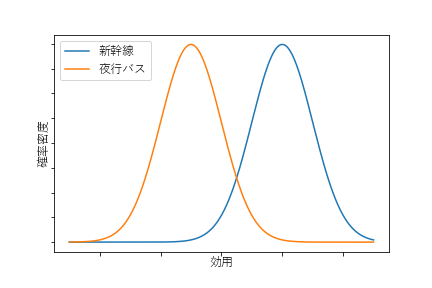
\includegraphics[width=0.5\hsize]{figure/norm1.png}
    \caption{新幹線と夜行バスの効用の比較}
    \label{fig:norm1}
\end{figure}

Aさんにとっては新幹線の方が効用が大きくなる可能性が高く、新幹線が選ばれる確率が高そうです。しかし、必ず新幹線が選ばれるとは限りません。

以下、Aさんにとっての新幹線の効用を $U_S$ 、夜行バスの効用を $U_B$ と書くことにします。$U_S,U_B$ は確率変数になります。ここでは $U_S,U_B$ が\textbf{独立であることを仮定}します。

このとき、Aさんが新幹線を選択する確率は、 $U_S$ が $U_B$ より大きくなる確率であり、 $P(U_S-U_B \geq 0)$ と書くことができます。$U_S$ と $U_B$ が正規分布に従う場合、 $U_S-U_B$ も正規分布に従う\footnote{正規分布の和・差の再生性として知られています。}ため、$P(U_S-U_B \geq 0)$ の値は正規分布の累積確率として求めることができます。

ここに第三の選択肢、飛行機を加えます。この時の効用は図\ref{fig:norm2}のようになります。

\begin{figure}[ht]
    \centering
    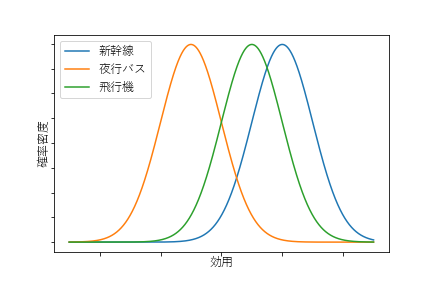
\includegraphics[width=0.5\hsize]{figure/norm2.png}
    \caption{新幹線と夜行バスと飛行機の効用の比較}
    \label{fig:norm2}
\end{figure}


Aさんにとっての飛行機の効用を $U_P$ と書くことにします(当然これも確率変数です)。このとき、この3つの選択肢の中からAさんが新幹線を選択する確率は、 $U_S$ が $U_B$ と $U_P$ より大きくなる確率であり、$P(U_S-U_B \geq 0 \land U_S-U_P \geq 0)$ と書くことができます。また、これを書き換えて $P(U_S - \max(U_B,U_P) \geq 0)$ とすることもできます。

$U_S,U_B,U_P$ が正規分布に従う場合、この確率を計算するのは簡単ではありません。$\max(U_B,U_P)$ が正規分布に従わないため、多重積分によって累積確率を求める必要があるからです。

このように、値を求めるのに積分計算が必要になるような式のことを\textbf{開形式}といい、数値計算上処理が重くなることから嫌われます。先ほどの選択肢が二つしかないバージョンも、正規分布の累積確率を計算するには積分が要るため、開形式です。

選択肢が二つ(二項)の場合であれば、単なる正規分布の累積確率なので数値計算ライブラリを使えば高速に値を求めることができますが、選択肢が三つ以上(多項)で多重積分が必要となると、計算時間が実用上問題になってくる恐れがあります。また数値積分なので誤差の懸念もあります。

そこで、\textbf{正規分布に似た形状の分布を正規分布の代わりに用いる}ことで、積分計算なしで選択確率を計算することが考えられました。

\subsection{ロジットモデル}\label{ssec:logit}

正規分布に形状が似ていて、離散選択モデルの計算上都合がいい性質を持っている分布として、\textbf{ガンベル分布}が用いられます。効用がガンベル分布に従うと仮定したモデルのことを\textbf{ロジットモデル}と呼びます。

ガンベル分布の確率密度関数 $f(x)$ は式(\ref{eq:gumbel_pdf})の通りです。

\begin{equation}
    \label{eq:gumbel_pdf}
    f(x) = \mu \exp(-\mu (x-\eta)) \exp(-\exp(-\mu (x-\eta)))
\end{equation}

また、累積密度関数は式(\ref{eq:gumbel_cdf})の通りです。

\begin{equation}
    \label{eq:gumbel_cdf}
    F(x) = \exp(-\exp(-\mu (x-\eta)))
\end{equation}

ここで、$\mu$ はガンベル分布の\textbf{スケールパラメータ}、$\eta$ は\textbf{ロケーションパラメータ}と呼ばれます。正規分布において平均値 $\mu$ と分散 $\sigma^2$ が与えられれば分布の形状が分かるのと同様に、ガンベル分布においてスケールパラメータとロケーションパラメータが分かれば分布の形状が分かります。

スケールパラメータ $\mu$ は分布のばらつきを意味する値であり、$\mu>0$ でなければいけません。$\mu<0$ だと確率密度関数が負値になってしまいます。

ロケーションパラメータ $\eta$ は分布の最頻値に一致します。

ガンベル分布は、2つの都合の良い性質を示します。

\begin{theorem}
    \label{it:gumbel_max}
    互いに独立な確率変数 $X_1,X_2, \ldots X_i, \ldots, X_N$ が,それぞれガンベル分布\mbox{}\\ $Gb(\eta_1, \mu), Gb(\eta_2, \mu),\ldots,Gb(\eta_i, \mu),\ldots,Gb(\eta_N, \mu)$ に従うとき、$\max(X_1,X_2, \ldots X_i, \ldots, X_N)$ は式(\ref{eq:gumbel_max})に示すパラメータを持つガンベル分布に従う。
    \begin{equation}
        \label{eq:gumbel_max}
        \left(\frac{1}{\mu} \ln\sum_{i=1}^N \exp(\mu\eta_i), \mu\right)
    \end{equation}

    ※ロケーションパラメータは変数ごとに異なっていてもよいですが、\textbf{スケールパラメータは同じ}である必要があります。
\end{theorem}
\begin{proof}
    \ref{prf:gumbel_max}を参照。
\end{proof}

\begin{theorem}
    \label{it:logistic}
    独立な二つの確率変数 $X_1,X_2$ がそれぞれガンベル分布 $Gb(\eta_1, \mu), Gb(\eta_2, \mu)$ に従うとき、その差 $X_1-X_2$ は、式(\ref{eq:logistic})に示す累積分布関数を持つ\textbf{ロジスティック分布}に従う。
    \begin{equation}
        \label{eq:logistic}
        F(x)=\frac{1}{1+\exp(\mu(\eta_1-\eta_2-x))}
    \end{equation}
\end{theorem}
\begin{proof}
    \ref{prf:logistic}を参照。
\end{proof}

この二つの性質を用いることで、積分計算なしに選択確率を計算することができます。

効用 $U_S,U_B,U_P$ が互いに独立でガンベル分布に従うとするとき、新幹線の選択確率 $P(U_S - \max(U_B,U_P) \geq 0)$ を計算します。

まずここで、3つの交通手段の\textbf{効用が従うガンベル分布は、全てスケールパラメータが同一であることを仮定します}。以下、$U_S \sim Gb(V_S, \mu), U_B \sim Gb(V_B, \mu), U_P \sim Gb(V_P, \mu)$ であるとします。

すると定理\ref{it:gumbel_max}により、

\begin{equation}
    \max(U_B,U_P) \sim Gb\left(\frac{1}{\mu} \ln\left(\exp(\mu V_B)+\exp(\mu V_P)\right), \mu\right)
\end{equation}
となります。

ここで $V_S^*=\frac{1}{\mu} \ln\left(\exp(\mu V_B)+\exp(\mu V_P)\right)$ とおき、$U_S=V_S+\varepsilon_S, \max(U_B+U_P)=V_S^*+\varepsilon_S^*$ となるように $\varepsilon_S, \varepsilon_S^*$ を定めると、$\varepsilon_S, \varepsilon_S^*$ はいずれも $Gb(0,\mu)$ に従う確率変数になります。

なお、$V_S$ を\textbf{確定部分}、$\varepsilon_S$ を\textbf{誤差項}と呼ぶことがあります。選択肢の効用 $U$ は確定部分と誤差項の和で表されます。

定理\ref{it:logistic}を用いて、

\begin{equation}
    \begin{aligned}
        P(U_S - \max(U_B,U_P) \geq 0)
         & = P(V_S+\varepsilon_S-V_S^*-\varepsilon_S^* \geq 0)                                                             \\
         & = P(\varepsilon_S^*-\varepsilon_S \leq V_S-V_S^*)                                                               \\
         & = \frac{1}{1+\exp(\mu(V_S^*-V_S))}                                                                              \\
         & = \frac{\exp(\mu V_S)}{\exp(\mu V_S)+\exp(\mu V_S^*)}                                                           \\
         & = \frac{\exp(\mu V_S)}{\exp(\mu V_S)+\exp(\mu \cdot \frac{1}{\mu} \ln\left(\exp(\mu V_B)+\exp(\mu V_P)\right))} \\
         & = \frac{\exp(\mu V_S)}{\exp(\mu V_S)+\exp(\mu V_B)+\exp(\mu V_P)}                                               \\
    \end{aligned}
\end{equation}


より一般に、$N$個の選択肢があって $i$ 番目の選択肢の効用が $Gb(V_i, \mu)$ に従うとき、$j$ 番目の選択肢が選択される確率は、以下の式(\ref{eq:mnl})で表されます。

\begin{equation}
    \label{eq:mnl}
    \frac{\exp(\mu V_j)}{\sum_{i=1}^N \exp(\mu V_i)}
\end{equation}

最後にもう一つ、$\mu=1$ \textbf{であると仮定}すれば、選択確率は以下の式(\ref{eq:mnl_one})で表されます。分子分母を $\mu$ で割ったわけではないことに注意してください。

\begin{equation}
    \label{eq:mnl_one}
    \frac{\exp(V_j)}{\sum_{i=1}^N \exp(V_i)}
\end{equation}

ロジットモデル、特に項が3つ以上の\textbf{多項ロジットモデル(MNL)}では、各選択肢の効用の確定部分 $V_i$ さえわかれば、式(\ref{eq:mnl})や式(\ref{eq:mnl_one})のような平易な式で各選択肢の選択確率を求めることができます。積分が不要な\textbf{閉形式}になっているため、実用上も高速です。

\section{仮定の整理}\label{sec:assumption}

上の選択確率の式(\ref{eq:mnl_one})を導くために、様々な仮定をおいてきました。モデルを実際に適用する際には、これらの仮定がそもそも成り立っているとみなしてよいのか、十分に注意する必要があります。以下、この章でおいた仮定を列挙します。

\begin{enumerate}
    \item 人は効用を最大にする選択肢を選ぶ。
    \item 効用にはランダム性があるが、その分布はガンベル分布に従う。
    \item 各選択肢の効用の分布は互いに独立である。
    \item 効用が従うガンベル分布のスケールパラメータはどの選択肢でも同じである。すなわち、効用のばらつきはどの選択肢でも同じである。
          \begin{itemize}
              \item これは効用の誤差項の分布が全て等しい($Gb(0,\mu)$ に従う)ことを意味する。
              \item 3番目の仮定と合わせて、各選択肢の効用の誤差項は互いに独立かつ同分布であり、このような条件を \textbf{IID} (Independent and Identically Distributed, 独立同分布) と呼ぶ。
          \end{itemize}
    \item スケールパラメータ $\mu=1$ である。
\end{enumerate}

\section{IIA特性}\label{sec:iia}

最後に、ロジットモデルの\textbf{IIA特性}に触れます。

IIA (Independence from Irrelevant Alternatives) 特性とは、二つの選択肢の間の選択確率の比は、その二つの選択肢の効用のみによって決まるという性質のことです。例えばMNLでは二つの選択肢 $i, j$ の間の選択確率の比は $\exp(V_i):\exp(V_j)$ と表されるため、確かにIIA特性を持っているといえます。ロジットモデルのIIA特性は、各選択肢の効用の分布が互いに独立であるという仮定によって生じたものです。

効用の分布が相関するような(似ている)選択肢がある場合、MNLにおける選択確率の計算結果が期待されるものと大きく異なってしまうことがあります。この問題は「\textbf{赤バス青バス問題}」と呼ばれています。

赤バス青バス問題は、次のような問題です。

\begin{itembox}[l]{赤バス青バス問題}
    「車」「赤バス」の二つの選択肢から選ぶロジットモデルにおいて、効用の確定部分が全く同じであれば、両者の選択確率は $1/2, 1/2$ となる。ここに「青バス」という選択肢を加えたとき、これの効用の確定部分も他と同じであったとすれば、三つの選択肢の選択確率は $1/3, 1/3, 1/3$ となる。色違いのバスが登場しただけでもともと車を利用していた人の三分の一もがバスに流れるのはおかしい。
\end{itembox}

赤バス青バス問題は、車と赤バスの選択確率の比が、青バスの有無によらず $1:1$ であるというIIA特性によって生じる問題です。

MNLで選択確率を適切に推定するには、選択肢の中で互いに似ているものがないことが必要です。赤バス青バス問題が起こりそうな場合には、\textbf{Nested Logit モデル}などのより応用的なモデルを用いることになります。

\chapter{効用関数}\label{ch:utility}

\ref{ch:model}章では、各選択肢の効用の確定項 $V$ が分かれば、各選択肢の選択確率が計算できることを示しました。この章では、多項ロジットモデルにおいて効用の確定項 $V$ をどのように求めるかを示します。

\section{効用の立式}\label{sec:utility}

まず、\textbf{効用は連続変数であり、いくつかの説明変数の線形和であることを仮定}します。

\textbf{説明変数}とは、各選択肢の定量可能な変数のことを指します。\ref{sec:utility_maxim}節で、効用の値はその選択肢の性質や選択行動をする個人の属性によって変わると書きました。例えば手段選択モデルの場合、下記のようなものが説明変数になりえます。

\begin{itemize}
    \item 所要時間
    \item 運賃
    \item 乗り換え回数
    \item 年齢
    \item 免許を持っているかどうか(持っていれば $1$, 持っていなければ $0$)
    \item ある交通手段の定期券を持っているかどうか
\end{itemize}

説明変数は大きく分けて、それぞれの交通手段に固有の特性と、選択をする個人の属性の2種類あるといえます。

これらの説明変数は、もちろん単位もバラバラですし、何よりどの指標がどれだけ効用に強く影響するかは分かりません。そこで、これらの説明変数をただ足し上げるのではなく、各説明変数に「\textbf{重み}」を掛けてから足し上げる必要があります。

例えば、東京から大阪へ行く選択肢が「新幹線」「夜行バス」「飛行機」の三択で、各選択肢の効用が「所要時間」「運賃」「年齢」で決まるとします。このときの新幹線の効用は、$x_{S,time}, x_{S,cost}, x_{age}$\footnote{個人の属性は選択肢によって変わることはないので、$x_{S,age}$ ではなく $x_{age}$ です。} がそれぞれ新幹線の所要時間・新幹線の運賃・個人の年齢であるとすると、以下の式(\ref{eq:utility_sample_train})のようにおくことができます。

\begin{equation}
    \label{eq:utility_sample_train}
    V_S=\beta_{time}x_{S,time}+\beta_{cost} x_{S,cost}+\beta_{S,age}x_{age}
\end{equation}

式(\ref{eq:utility_sample_train})の $\beta$ が「重み」に相当する値で、未知のパラメータです。

同様に、夜行バスと飛行機の効用も式にしてみます。

\begin{align}
    V_B & =\beta_{time}x_{B,time}+\beta_{cost} x_{B,cost}+\beta_{B,age}x_{age} \label{eq:utility_sample_bus}      \\
    V_P & =\beta_{time}x_{P,time}+\beta_{cost} x_{P,cost}+\beta_{P,age}x_{age} \label{eq:utility_sample_airplane}
\end{align}

所要時間のパラメータ $\beta_{time}$ と運賃のパラメータ $\beta_{cost}$ は3つの式(\ref{eq:utility_sample_train})(\ref{eq:utility_sample_bus})(\ref{eq:utility_sample_airplane})で共通なのに対し、年齢のパラメータは選択肢ごとに $\beta_{S,age}, \beta_{B,age}, \beta_{P,age}$ と別の変数になっている点に注目してください。

所要時間や運賃など交通手段に固有の特性に掛ける重みは、すべての選択肢で同じにすることで、その特性がどう選択に影響するかを表すことができます。例えば、$\beta_{time}$ が負の値であれば、時間がかかるほど($x_{S,time}, x_{B,time}, x_{P,time}$ が大きくなるほど)効用が小さくなるということを意味します。

一方、個人の属性に掛ける重みは、選択肢ごとに分けることで、その属性の持ち主が相対的にどの選択肢を選びやすくなるかを表すことができます。例えば、$\beta_{B,age}<\beta_{P,age}$ ならば、年齢が高いほど($x_{age}$ が大きくなるほど)相対的に飛行機の方が効用が大きくなるということを意味します。

また、これらの説明変数では説明できない、各選択肢に固有の好まれ具合を表現するために、最後に説明変数を掛けないパラメータを付けます。なおこのとき、\textbf{「説明変数を掛けないパラメータ」を全ての選択肢につけてはいけません。}理由はこの後の\ref{ssec:est_unique}項で説明します。

\begin{align}
    V_S & =\beta_{time}x_{S,time}+\beta_{cost} x_{S,cost}+\beta_{S,age}x_{age}         \\
    V_B & =\beta_{time}x_{B,time}+\beta_{cost} x_{B,cost}+\beta_{B,age}x_{age}+\beta_B \\
    V_P & =\beta_{time}x_{P,time}+\beta_{cost} x_{P,cost}+\beta_{P,age}x_{age}+\beta_P
\end{align}

\subsection{より複雑な立式}

\begin{itemize}
    \item 「免許を持っていない人は絶対に車で移動しない」といったことを表現するには、$V_{car}=-\infty$ とすればよいです。こうすることで選択確率 $\frac{\exp(V_{car})}{\sum \exp V}$ の分子が強制的に $0$ になり、選択確率が $0$ すなわち絶対に選択されない状態になります。

    \item 説明変数の $\log$ などをとってから重みを掛けるという方法もあり得ます。「所要時間が20分から15分になった」場合と「所要時間が120分から115分になった」場合で、どちらも同じだけ効用が増加したと考えるよりは、20分→15分の方が効用の増加幅が大きいとする方が自然でしょう。$\log$ を取るなどすることでこのような非線形な効用の増減も表現できます。

          ただし、このような調整を恣意的に行うことは Data dredging や p-hacking 等と呼ばれ、研究不正にあたります。\textbf{行動メカニズムとして説明できないような効用式を立ててはいけません}。
\end{itemize}

\chapter{パラメータ推定}\label{ch:parameter_est}

\ref{ch:utility}章で立式した効用の値を求めるには、未知のパラメータである $\beta_{time}, \beta_{cost}, \beta_{S,age}, \ldots$ を求めなければいけません。これらの未知パラメータを、データを使って推定することを\textbf{パラメータ推定}といいます。

パラメータ推定では、パラメータの\textbf{尤度}(もっともらしさ)が最大になるようにパラメータを決定します。離散選択モデルの場合、\textbf{モデルから計算される各選択肢の選択確率が、実際の各選択肢の選択確率にできるだけ近くなるように}すればよいです。

\section{パラメータ推定に用いるデータ}\label{sec:data}

実際の各選択肢の選択確率は、交通分野の場合、以下のようなデータを組み合わせて用いることで得ることができます。

\begin{description}
    \item[LOSデータ]交通サービス水準。所要時間や運賃など交通手段に固有の特性を表すデータ。
    \item[RP調査によるデータ]人々がある地点から別の地点へ実際に移動する際に、いつ・どこへ・どんな交通手段で・何のために移動したのかの情報を収集したデータ。個人の属性の情報もセットで記録する。
    \begin{description}
        \item[PT(パーソントリップ)データ] RP調査のうち、平均的な一日の行動についてアンケートによって収集したデータ。
        \item[PP(プローブパーソン)データ] RP調査のうち、GPS等を用いて実際の行動記録を収集して整理したデータ。
    \end{description}
    \item[SP調査によるアンケートデータ]様々な条件を仮定したときにどんな移動をすることを選ぶかの希望を、アンケートによって収集したデータ。実際の行動に基づかないためやや信頼性が落ちる代わりに、未来の交通手段などを想定したアンケートをすることができる。個人の属性の情報もセットで記録する。LOSに相当する、どの選択肢ならどんな条件で使えるかという情報がアンケート内に含まれている。
\end{description}


これらのデータから、交通手段に固有の特性や個人の属性といった説明変数になりえる値と、実際にどの選択肢が選ばれたかという結果がわかります。パラメータ推定によってモデルを実際の選択結果に近づけ、できたモデルをもとに新たな条件ではどの選択肢がどれだけの確率で選択できるかを推定する、というのがモデルの活用の流れです。

\section{尤度}\label{sec:likelihood}

MNLにおける尤度の求め方を示します。

$M$ 人が $N$ 個の選択肢の中から独立に選択行動をします。$i$ 番目の人にとっての説明変数が $\bm{x_i}$ である\footnote{説明変数は複数個ありうるのでベクトルで表記します。ここでは、交通手段の特性由来の説明変数も、個人の属性由来の説明変数も一つにまとめています。}とき、選択肢 $y_i$ が選ばれる確率を $P(y_i;\bm{x_i})$ と書くことにします。

このとき $1,2,\ldots,M$ 番目の人が それぞれ $y_1,y_2,\ldots,y_M (1 \le y_i \le N)$ の選択肢を選択する同時確率は、各人の選択行動が独立であることから、式(\ref{eq:joint_prob})のように表されます。

\begin{equation}
    \label{eq:joint_prob}
    P(y_1;\bm{x_1},y_2;\bm{x_2},\ldots,y_M;\bm{x_M}) = P(y_1;\bm{x_1})P(y_2;\bm{x_2}) \cdots P(y_M;\bm{x_M}) = \prod_{i=1}^M P(y_i;\bm{x_i})
\end{equation}

なお、MNLでは式(\ref{eq:joint_prob})の値は次の式(\ref{eq:joint_prob_mnl})のように書けます。

\begin{equation}
    \label{eq:joint_prob_mnl}
    \prod_{i=1}^M\frac{\exp(V_{y_i})}{\sum_{j=1}^N \exp(V_j)}
\end{equation}

効用の確定項 $V$ は、\ref{ch:utility}章で立式したように、説明変数 $\bm x$ と未知パラメータ $\bm\beta$ \footnote{未知パラメータも複数あるのでベクトルで表記します。}によって決まる値でした。

ところで、$i$ 番目の人が $y_i$ を選ぶという事象はすでに確定していますし、各人・各選択肢の説明変数も分かっています。分かっていない値は未知パラメータです。そこで\textbf{尤度関数} $L(\bm\beta)$ を、式の形は変えずに次のように定義します。

\begin{equation}
    \label{eq:likelihood}
    L(\bm\beta) \coloneq \prod_{i=1}^M P(y_i;\bm{x_i}) = \prod_{i=1}^M\frac{\exp(V_{y_i})}{\sum_{j=1}^N \exp(V_j)}
\end{equation}

すると、この尤度関数を最大化することは、$\bm\beta$ を変化させることによって $y_1,y_2,\ldots,x_M$ の選択肢が選択される同時確率を最大化することにほかなりません。したがって、尤度関数を最大化するような $\bm\beta$ と、$\bm\beta$ によって計算される効用の確定項 $V$ は、実際の現象をもっともうまく表現しているということができます。

このように、尤度を最大化するようなパラメータを真のパラメータであるとする手法のことを\textbf{最尤推定法}といいます。

ある条件においてどの選択肢がどのくらいの確率で選ばれるのかを推定する、という問題は、最終的に関数を最大化する問題に帰着されました。関数の最大化問題は、古くから数理最適化の分野で研究が進められ、強力なソルバーが多数提供されています。よって、この関数の最大化問題には深く立ち入らず、実装上はRやPythonのSciPyで提供されている\textbf{最適化ライブラリ}を使用して解きます。

ライブラリに投げる前に、2点注意するべきことがあります。1つは尤度を直接最大化する代わりに次項で述べる\textbf{対数尤度}を最大化すること、もう1つは最尤推定法によって未知パラメータが一意に定まるように効用を立式することです。

\subsection{対数尤度}\label{ssec:log_likelihood}

対数尤度とは、尤度の対数を取った値です。尤度 $L(\bm\beta) = \prod_{i=1}^M P(y_i;\bm{x_i})$ は、1より小さい値を大量に掛け合わせて得られるため、非常に小さな値をとります。このため、プログラムで尤度を直接求めると、誤差によって $0$ に丸められてしまう恐れがあります。

そこで、尤度を最大化する代わりに尤度の対数を取った値を最大化することを考えます。対数尤度 $LL(\bm\beta)$ は次の式(\ref{eq:log_likelihood})で定義されます。

\begin{equation}
    \label{eq:log_likelihood}
    LL(\bm\beta) \coloneq\log L(\bm\beta) = \sum_{i=1}^M \log P(y_i;\bm{x_i})
\end{equation}

対数尤度の値は、選択確率が非常に小さくなるような選択肢が選ばれていない限りは問題なく計算できます。

\subsection{未知パラメータが一意に定まるような効用式}\label{ssec:est_unique}

尤度が最大となるようなパラメータの組が無限通りある、という状況が生じてしまうと、尤度関数の最大化が収束しなくなりパラメータ推定に失敗してしまいます。

例えば、効用の確定項を下の式(\ref{eq:utility_bad})のように立式すると、パラメータ推定に失敗します。

\begin{equation}
    \label{eq:utility_bad}
    \begin{aligned}
        V_S & =\beta_{time}x_{S,time}+\beta_{cost} x_{S,cost}+\beta_{S,age}x_{age}+\beta_S \\
        V_B & =\beta_{time}x_{B,time}+\beta_{cost} x_{B,cost}+\beta_{B,age}x_{age}+\beta_B \\
        V_P & =\beta_{time}x_{P,time}+\beta_{cost} x_{P,cost}+\beta_{P,age}x_{age}+\beta_P
    \end{aligned}
\end{equation}

「説明変数を掛けないパラメータ」を全ての選択肢につけてはいけません。次の式(\ref{eq:utility_good})のように,\textbf{「説明変数を掛けないパラメータ」の数は、選択肢の数よりも1少なくなるようにする}必要があります。

\begin{equation}
    \label{eq:utility_good}
    \begin{aligned}
        V_S & =\beta_{time}x_{S,time}+\beta_{cost} x_{S,cost}+\beta_{S,age}x_{age}         \\
        V_B & =\beta_{time}x_{B,time}+\beta_{cost} x_{B,cost}+\beta_{B,age}x_{age}+\beta_B \\
        V_P & =\beta_{time}x_{P,time}+\beta_{cost} x_{P,cost}+\beta_{P,age}x_{age}+\beta_P
    \end{aligned}
\end{equation}

選択確率の式(\ref{eq:mnl})を見ればわかるように、選択確率は $V$ の値そのものではなく、$\exp(V)$ の値の\textbf{比}によって決まります。「説明変数を掛けないパラメータ」をすべての選択肢の効用式につけると、各選択肢の選択確率が同じになるような $(\beta_S, \beta_B, \beta_P)$ の値の組が無限通り存在することになってしまいます。説明変数を掛けないパラメータを一つ減らすことで自由度が下がり、この問題が解消されます。

\chapter{検定}\label{ch:testing}

\ref{ch:parameter_est}章までで、多項ロジットモデルを作って各選択肢の選択確率を求めることができるようになりました。

しかし、最尤推定法によって尤もらしいパラメータを推定することができたからといって、そのパラメータが統計的に信頼できるとは限りません。また、そのパラメータと説明変数を持つモデルが実際のデータにどのくらいうまく適合しているかも知る必要があります。

例えば、もし所要時間の重みパラメータ $\beta_{time}$ の推定値が統計的に信頼できないとみなすならば、そのモデルを使って所要時間の変化に伴う乗客数の変化を推定することはできません。また、新しい説明変数とパラメータを追加することでモデルの適合度が\textbf{有意に}向上するのであれば、新しいモデルの方を採用するべきでしょう。

求めたパラメータが統計的に信頼できるかどうかを判定するための方法の一つとして、\textbf{t検定}がしばしば用いられます。また、モデルと実際のデータの適合度合いを見るために\textbf{尤度比検定}が用いられます。

\section{t検定}\label{sec:t_test}

ここでは、紛らわしい統計用語を順を追って整理し、最終的にt検定について説明します。

\subsection{統計量}\label{ssec:statistic}

統計的分析の対象となる人や物事の集まりを\textbf{母集団}、母集団から抽出してきた人や物事の集まりを\textbf{標本}といいます。標本に対して、標本に関する何らかの値(選択行動の結果など)を取り出してくると、その値は標本の選び方によって変わる\textbf{確率変数}になります。このようにして得られる確率変数の集まりのことを\textbf{標本変量}といいます。

\textbf{統計量}とは、標本変量に対して何らかの操作を行うことによって得ることができる、その標本変量の特徴を簡潔に示す量のことです。例えば算術平均は「標本変量の総和を標本数で割る」という操作によって得ることができる統計量です。また分散、中央値、最頻値なども同様に統計量です。

重要な事実として、標本変量は確率変数の集まりなので、それに対して操作を加えて得られる\textbf{統計量もまた確率変数}です。

\subsection{推定値と推定量}\label{ssec:estimator}

\ref{sec:likelihood}節では最尤推定法によって未知パラメータ $\bm\beta$ の値を推定しました。このときは実際に観測されたデータを使って推定を行ったので $\bm\beta$ の具体的な値を求めることができました。これを $\beta$ の\textbf{推定値}と呼びます。特にこの場合は最尤推定法によって得られた値なので、\textbf{最尤推定値}と呼びます。しかし、最尤推定値の値は標本の選び方によって変わるはずです。

最尤推定の結果は、標本変量に対して尤度を最大化するという操作を行うことで得られる量なので、統計量の定義を満たしています。このように、何らかの推定のために得る統計量のことを\textbf{推定量}と呼び、$\hat\beta$ と記します。特にこの場合は最尤推定法によって得られた推定量なので、\textbf{最尤推定量}と呼びます。最尤推定量は統計量なので確率変数であり、したがって確率分布を持ちます。

t検定では、「各パラメータの最尤推定量がとる値が $0$ になる確率」を計算します。$i$ 番目のパラメータ $\beta_i$ の真の値が $0$ であるとき、そのパラメータに対応する説明変数 $x_i$ に何を代入しても効用の値が変化しないので、その説明変数は選択行動を説明するのに全く役立たないということになります。逆にこのようなことになる確率が十分に低ければ、そのパラメータに対応する説明変数 $x_i$ は選択行動を説明しているということができます。

なお、最尤推定量は以下の性質を満たします。

\begin{description}
    \item[一致性] 無限個の標本を用いて推定した最尤推定値は、パラメータの真値に一致する。
    \item[漸近正規性] 標本が多く\footnote{50件とか100件以上などと言われています。}なると、最尤推定量の分布は正規分布に近づく。
    \item[漸近有効性] 標本が多くなると、最尤推定量の分散は\textbf{クラメール・ラオの不等式}の下限に近付く。
\end{description}

\subsection{最尤推定量の分散}\label{ssec:variance_estimator}

推定量の期待値がパラメータの真値に一致するとき、その推定量は\textbf{不偏推定量}であるといいます(一致性とは異なる概念です)。さらに、その不偏推定量が他のどの不偏推定量よりも分散が大きくないとき、その推定量は\textbf{有効推定量}であるといいます。最尤推定量は不偏推定量ではないので、当然有効推定量でもありませんが、標本が多くなると漸近的に有効推定量のようなふるまいを見せる、というのが漸近有効性です。

有効推定量が定義可能であることからも分かるように、不偏推定量の分散には下限が存在します。この不偏推定量の分散の下限を示すのがクラメール・ラオの不等式です。

\begin{theorem}[クラメール・ラオの不等式]
    \label{it:cramer_rao}
    $\bm{\hat\beta}$ をパラメータ $\bm\beta$ の不偏推定量とし、$\cov(\bm{\hat\beta})$ は $\bm{\hat\beta}$ の分散共分散行列、$LL$ は対数尤度関数とする。このとき以下の行列に対する不等式が成り立つ。
    
    \begin{align}
        \label{eq:fisher_information}
        I(\bm\beta) \coloneqq -\mathbb{E}\left[\nabla\nabla^\top LL(\bm\beta)\right] \\  
        \label{eq:cramer_rao}
        \cov(\bm{\hat\beta}) \ge I(\bm\beta)^{-1}
    \end{align}
    ただし、式(\ref{eq:cramer_rao})の不等号は、左辺から右辺を引いた行列 $\cov(\bm{\hat\beta})-I(\bm\beta)^{-1}$ が半正定値行列であることを意味する\footnote{もし $\bm\beta$ が1変数のパラメータであれば、この不等号は単に実数の不等号と同じ意味になります。}。
\end{theorem}
\begin{proof}
    \ref{prf:cramer_rao}を参照。
\end{proof}

$I(\bm\beta)$は\textbf{フィッシャー情報行列}と呼ばれます。なお、$\nabla\nabla^\top LL(\bm\beta)$ は書き出すと下の式(\ref{eq:hessian_matrix})のようになり、特に行列部分には\textbf{ヘッセ行列}という名前がつけられています。

\begin{equation}
    \label{eq:hessian_matrix}
    \nabla\nabla^\top LL(\bm\beta) = \begin{bmatrix}
        \frac{\partial^2 LL}{\partial {\beta_1}^2}              & \frac{\partial^2 LL}{\partial \beta_1 \partial \beta_2} & \cdots & \frac{\partial^2 LL}{\partial \beta_1 \partial \beta_n}  \\
        \frac{\partial^2 LL}{\partial \beta_2 \partial \beta_1} & \frac{\partial^2 LL}{\partial {\beta_2}^2}              & \cdots & \frac{\partial^2 LL}{\partial \beta_2 \partial \beta_n } \\
        \vdots                                                  & \vdots                                                  & \ddots & \vdots                                                   \\
        \frac{\partial^2 LL}{\partial \beta_n \beta_1}          & \frac{\partial^2 LL}{\partial \beta_n \partial \beta_2} & \cdots & \frac{\partial^2 LL}{\partial {\beta_n}^2}
    \end{bmatrix} \bm\beta
\end{equation}

等号が成立する時、$\bm{\hat\beta}$ は分散の下限を達成しているので、$\bm{\hat\beta}$ は有効推定量となります。最尤推定量の場合は、漸近有効性により、標本が十分多ければ等号成立、すなわち

\begin{equation}
    \label{eq:fisher_information_inv}
    \cov(\bm{\hat\beta}) \simeq I(\bm\beta)^{-1}
\end{equation}

としてよいです。このように、フィッシャー情報行列を求めることで、最尤推定量の分散を求めることができます。

フィッシャー情報行列を確率変数である$\bm\beta$の分布から直接計算することもできますが、フィッシャー情報行列に代えて\textbf{観測された情報行列}を用いる方が計算が簡単かつ有用です\cite{Efron1978}。観測された情報行列$J(\bm{\hat\beta})$は次のように定義されます。

\begin{equation}
    \label{eq:observed_information}
    J(\bm{\hat\beta}) \coloneqq -\nabla\nabla^\top LL(\bm{\hat\beta})
\end{equation}

式(\ref{eq:observed_information})を用いると、式(\ref{eq:fisher_information_inv})の代わりに次の式が得られます。

\begin{equation}
    \label{eq:observed_information_inv}
    \cov(\bm{\hat\beta}) \simeq J(\bm{\hat\beta})^{-1}
\end{equation}

\subsection{区間推定}\label{ssec:interval_est}

t検定では、各パラメータについて、次のような\textbf{帰無仮説}を立てます。

\begin{itembox}[l]{t検定での帰無仮説}
    パラメータ $\beta_i$ の最尤推定量 $\hat\beta_i$ がとる値は $0$ である。
\end{itembox}

この帰無仮説が一定の\textbf{有意水準}で\textbf{棄却}されるならば、パラメータ $\beta_i$ の最尤推定量が $0$ とは有意に異なるとみなすことができます。

帰無仮説が棄却されるかどうかを調べるためには、$\beta_i$ の最尤推定量がとりうる区間を推定し、$0$ が\textbf{信頼区間}内に入ってこないことを確認すればよいです。

\begin{figure}[ht]
    \centering
    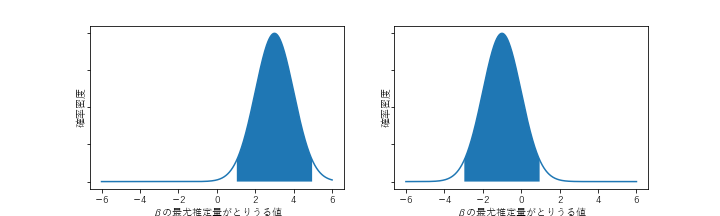
\includegraphics[width=0.9\hsize]{figure/interval_estimation.png}
    \caption{信頼区間}
    \label{fig:interval_est}
\end{figure}


図\ref{fig:interval_est}で青く塗っている区間が信頼区間です。例えば「$95\%$ 信頼区間」であれば、パラメータ $\beta_i$ の最尤推定量 $\hat\beta_i$ がとる値が $95\%$ の確率でその区間内に収まることを意味します。

左の図では、$95\%$ 信頼区間内に $0$ が含まれていないので、$\hat\beta_i$ が取る値が $0$ になる確率は $5\%$ 以下となります。すると「パラメータ $\beta_i$ の最尤推定量 $\hat\beta_i$ がとる値は $0$ である」という帰無仮説は $5\%$ 有意水準で棄却されることになり、そのパラメータに対応する説明変数は選択行動を説明しているということができます。

いっぽう右の図では、$95\%$ 信頼区間内に $0$ が含まれているので、帰無仮説は棄却されません。すると、そのパラメータに対応する説明変数が選択行動を説明しているかどうかは分かりません(\textbf{説明変数が「効かない」ことを意味しているわけではなく、「効くとは言い切れない」ということを意味します})。

ここで、信頼区間の幅を求めるには、最尤推定量の分散が必要になります。最尤推定量の分散を求めるために式(\ref{eq:observed_information_inv})を用います。なお$L$ のヘッセ行列は数値微分によって計算できます。

各パラメータの最尤推定量の分散 $\bm s^2$ が分かれば、最尤推定量の漸近正規性により、正規分布の場合と同様に信頼区間を求めることができます。

各パラメータの最尤推定量を $t_i\coloneq\frac{\hat\beta_i}{s}$ と標準化します。このとき出現する値 $t_i$ は\textbf{t値}と呼ばれ、t値が\textbf{標準正規分布}の $95\%$ 信頼区間内に入っていないならば、帰無仮説は $5\%$ 有意水準で棄却されることになります。このようなt値の閾値は $|t|>1.96$ です(標準正規分布の両側 $5\%$ 点は $1.96$)。また、$|t|>2.58$ となれば帰無仮説は $1\%$ 有意水準で棄却されることになります。

\section{尤度比指標}\label{sec:likelihood_ratio}

\subsection{尤度比検定}

尤度比検定は、先ほどのt値とは異なり、あるモデルが全体として別のモデルより適合度が高いかどうかを見る検定です。

モデルAを、モデルBにいくつかの説明変数とパラメータを加えたモデルとします。モデルAとモデルBの尤度比は、文字通り尤度の比 $\frac{L(\bm{\hat\beta_A})}{L(\bm{\hat\beta_B})}$ です。尤度比の対数は $LL(\bm{\hat\beta_A})-LL(\bm{\hat\beta_B})$ となり、対数を取った方の値を単に\textbf{尤度比}と呼ぶことがあります。尤度比は確率変数なので検定可能です。

尤度比検定では、次のような帰無仮説を立てます。

\begin{itembox}[l]{尤度比検定での帰無仮説}
    帰無仮説:モデルAとモデルBの尤度比は $0$ である。
\end{itembox}

尤度が大きい方がより「もっともらしい」モデルなので、説明変数が多いモデルAの方が尤度が大きくなってほしいところです。この帰無仮説が棄却されればモデルAの方が有意に尤度が大きいということができ、二つのモデルの適合度の差が有意なものであるということができます。

ところで、標本が十分多いとき、尤度比を $2$ 倍した値は\textbf{カイ二乗分布}と呼ばれる分布に従うことが知られています。特に、$\bm\beta_A$ のパラメータ数が $N_A$ 個、$\bm\beta_B$ のパラメータ数が $N_B$ 個であるとき、 $2(LL(\bm{\hat\beta_A})-LL(\bm{\hat\beta_B}))$ は\textbf{自由度} $N_A-N_B$ のカイ二乗分布に従います。

したがって、帰無仮説「モデルAとモデルBの尤度比は $0$ である」を棄却するには、$2(LL(\bm{\hat\beta_A})-LL(\bm{\hat\beta_B}))$ の信頼区間内に $0$ が入ってこないことを示せばよいです。

たとえば $N_A=7, N_B=5$ のとき、自由度 $2$ のカイ二乗分布の上側 $5\%$ 点は $5.99$ なので、$2(LL(\bm{\hat\beta_A})-LL(\bm{\hat\beta_B}))>5.99$ ならば $5\%$ 有意水準で帰無仮説が棄却されることになります。

特に、すべての選択肢の効用を $0$ としたモデル(説明変数もパラメータもないモデル)をモデルBとして尤度比検定することで、作ったモデルの適合度が有意であることを確認することができます。すべての選択肢の効用を $0$ としたモデルのことを \textbf{Null model} と呼び、その対数尤度は $LL(\bm 0)$ で求めることができます。

注意すべき点として、モデルAはモデルBを含んでいる、上位互換のモデルである必要があります。厳密に述べると、モデルAに含まれない説明変数・パラメータであって、モデルBに含まれるような説明変数・パラメータがあってはいけません。

\subsection{McFaddenの擬似決定係数}

尤度比検定では、尤度比をカイ二乗分布の上側 $5\%$ 点と比較することで、モデルの適合度が有意であるかどうかを判定しました。しかし、カイ二乗分布の上側 $5\%$ 点は自由度によって変化するので、モデルの適合度が有意であるかどうかを判定するためには、モデルのパラメータ数に応じてカイ二乗分布の上側 $5\%$ 点を求める必要があります。回帰分析における決定係数のように、0から1の範囲に収まるより分かりやすい指標が欲しいところです。

そこで、\textbf{McFaddenの擬似決定係数}という指標が考案されました。McFaddenの擬似決定係数 $\rho^2$ は次のように定義されます。

\begin{equation}
    \rho^2 \coloneq \frac{LL(\bm 0)-LL(\bm{\hat\beta})}{LL(\bm 0)} = 1-\frac{LL(\bm{\hat\beta})}{LL(\bm 0)}
\end{equation}

この指標は $0$ から $1$ の範囲に収まるので、決定係数のようにモデルの適合度を示す指標として使うことができます。交通分野で\textbf{尤度比}といった場合、このMcFaddenの擬似決定係数のことを指す場合もあります。

整理すると、単に尤度比といった場合、次の三つの値のどれを指しているかは資料によって異なります。

\begin{enumerate}
    \item 2つのロジットモデルの尤度の比 $\frac{L(\bm{\hat\beta_A})}{L(\bm{\hat\beta_B})}$
    \item 2つのロジットモデルの対数尤度の差 $LL(\bm{\hat\beta_A})-LL(\bm{\hat\beta_B})$
    \item あるロジットモデルのMcFadden擬似決定係数 $\rho^2=1-\frac{LL(\bm{\hat\beta})}{LL(\bm 0)}$
\end{enumerate}

\subsection{自由度調整済み決定係数}

McFaddenの擬似決定係数は、モデルのパラメータ数に応じてカイ二乗分布の上側 $5\%$ 点を求める必要がないという利点がありますが、モデルのパラメータ数が多くなるほど指標値が増加するという欠点があります。そこで、\textbf{自由度調整済み決定係数}という指標が考案されました。

自由度調整済み決定係数 $\bar\rho^2$ は次のように定義されます。

\begin{equation}
    \bar\rho^2 \coloneq 1-\frac{LL(\bm{\hat\beta})-N}{LL(\bm 0)}
\end{equation}

$N$は未知パラメータの数です。

この指標はパラメータの数にかかわらず用いることができ、経験的に$0.2$以上であれば十分、$0.15$以上でもまあ良しとされます。

なお、自由度調整済み決定係数のことを\textbf{修正済み決定係数}と呼ぶこともあります。

ロジットモデルの推定を行った論文では、初期尤度(Null Model の対数尤度)$LL(\bm 0)$、最終尤度 $LL(\bm{\hat\beta})$ とともに、McFaddenの擬似決定係数や自由度調整済み決定係数が報告されることが多いです。報告の形式についてはこのあとの\ref{sec:est_result}節を参照してください。
\chapter{PythonによるMNLの実装}\label{code}

ここでは、\cite{binn}に付録されている MNLのRによる実装について、Pythonで書き換えたものを示します。

\section{ファイルの読み込み等}

\begin{lstlisting}[language=Python]
import numpy as np
import pandas as pd
from scipy.optimize import minimize
df = pd.read_csv('ensyu.csv', encoding='shift-jis')
\end{lstlisting}

パラメータ推定に用いるPTデータは、たいていの場合CSVで提供され、一行に一人分のデータが入っている、というようなフォーマットになっています。Pythonでこのようなデータを扱うにはPandasが便利です。

\section{効用の計算}

\begin{lstlisting}[language=Python]
def fr(x: np.array) -> float:
    b1, b2, b3, b4, d1, f1 = x  # b1~b4: 定数項, d1: 所要時間, f1: 運賃
    
    train: pd.Series = df["代替手段生成可否train"] * np.exp(
    d1 * df["総所要時間train"] / 100 + f1 * df["費用train"] / 100 + b1
    )
    bus: pd.Series = df["代替手段生成可否bus"] * np.exp(
    d1 * df["総所要時間bus"] / 100 + f1 * df["費用bus"] / 100 + b2
    )
    car: pd.Series = df["代替手段生成可否car"] * np.exp(
    d1 * df["総所要時間car"] / 100 + b3
    )
    bike: pd.Series = df["代替手段生成可否bike"] * np.exp(
    d1 * df["総所要時間bike"] / 100 + b4
    )
    walk: pd.Series = df["代替手段生成可否walk"] * np.exp(
    d1 * df["総所要時間walk"] / 100
    )

    # 続きます
\end{lstlisting}

「電車」「バス」「車」「自転車」「徒歩」から選択する手段選択モデルをつくります。効用関数は式(\ref{eq:utility_sample})の通りとしています。

\begin{equation}
    \label{eq:utility_sample}
    \begin{aligned}
         & V_{train} & = & \frac{\beta_{d1} x_{train, time}}{100} & + & \frac{\beta_{f1} x_{train, cost}}{100} & + \beta_1 \\
         & V_{bus}   & = & \frac{\beta_{d1} x_{bus, time}}{100}   & + & \frac{\beta_{f1} x_{bus, cost}}{100}   & + \beta_2 \\
         & V_{car}   & = & \frac{\beta_{d1} x_{car, time}}{100}   &   &                                        & + \beta_3 \\
         & V_{bike}  & = & \frac{\beta_{d1} x_{bike, time}}{100}  &   &                                        & + \beta_4 \\
         & V_{walk}  & = & \frac{\beta_{d1} x_{walk, time}}{100}                                                           \\
    \end{aligned}
\end{equation}



$\beta_{d1}$ が所要時間に関するパラメータ、$\beta_{f1}$ が運賃に関するパラメータ、それ以外の4つが定数項(説明変数に掛けないパラメータ)です。\ref{ssec:est_unique}項で見た通り、説明変数に掛けないパラメータの数は、選択肢の数より1少なくしないといけません。

このコードでは \lstinline{train} \lstinline{bus} などの変数に、効用の確定項そのものではなくその $\exp$ をとったものを代入しています。

$\exp$ をとったあとに \lstinline{df["代替手段生成可否train"]} などを掛けていますが、この列は「その選択肢が選択可能かどうか」を表しています(選択可能なら $1$, 不可なら $0$)。\ref{ch:utility}章の最後で少し触れていますが、選択確率を $0$ にしたいという場合には $V=-\infty$ とすればよく、このコードではその代わりに $\exp(V)=0$ としています。

なお、これらの変数は \lstinline{pd.Series} という型になっています。これらはそれぞれ人数分の長さを持つ一次元配列のようなものだと考えてください。

\section{選択確率の計算}

\begin{lstlisting}[language=Python]
def fr(x: np.array) -> float:
    # (前略)
    # 続き

    deno: pd.Series = car + train + bus + bike + walk

    Ptrain: pd.Series = df["代替手段生成可否train"] * (train / deno)
    Pbus: pd.Series = df["代替手段生成可否bus"] * (bus / deno)
    Pcar: pd.Series = df["代替手段生成可否car"] * (car / deno)
    Pbike: pd.Series = df["代替手段生成可否bike"] * (bike / deno)
    Pwalk: pd.Series = df["代替手段生成可否walk"] * (walk / deno)

    # 続きます
\end{lstlisting}

\lstinline{deno} には選択確率の分母となる $\sum_{i=1}^N \exp(V_i)$ の値を代入し、それを使って各選択肢の選択確率 $P_j=\frac{\exp(V_j)}{\sum_{i=1}^N \exp(V_i)}$ を計算しています。これで、各参加者がそれぞれどれだけの選択確率で選択肢を選ぶかが分かります。

    \section{対数尤度の計算}

    \begin{lstlisting}[language=Python]
def fr(x: np.array) -> float:
    # (前略)
    # 続き
    
    Ptrain = Ptrain.where(Ptrain != 0, 1)
    Pbus = Pbus.where(Pbus != 0, 1)
    Pcar = Pcar.where(Pcar != 0, 1)
    Pbike = Pbike.where(Pbike != 0, 1)
    Pwalk = Pwalk.where(Pwalk != 0, 1)
    
    Ctrain: pd.Series = df["代表交通手段"] == "鉄道"
    Cbus: pd.Series = df["代表交通手段"] == "バス"
    Ccar: pd.Series = df["代表交通手段"] == "自動車"
    Cbike: pd.Series = df["代表交通手段"] == "自転車"
    Cwalk: pd.Series = df["代表交通手段"] == "徒歩"
    
    LL: float = np.sum(
    Ctrain * np.log(Ptrain)
    + Cbus * np.log(Pbus)
    + Ccar * np.log(Pcar)
    + Cbike * np.log(Pbike)
    + Cwalk * np.log(Pwalk)
    )
    return LL
\end{lstlisting}


    選択肢を計算した後に、\lstinline{Ptrain = Ptrain.where(Ptrain != 0, 1)} のような処理が入っています。これは「選択確率が$0$ のときに $1$ に直す」という処理で、単に選択確率を出すだけならいらない(というよりやってはいけない)処理です。しかし、最後に対数尤度を計算する際に選択確率の $\log$ を取る必要があるため、選択確率に $0$ が含まれていると困ります。そこで $P=1$ にすることで、 $\log(1)=0$ を利用して $LL$ の値に影響を与えないようにすることができます。

    その次の \lstinline{Ctrain} などの変数には、「選択されたのが鉄道なら $1$ 、そうでないなら $0$」のような値が入ります。もちろんこれらも人によって選択結果が違うので、人数分の長さの配列になっています。

    最後の \lstinline{LL} の式が対数尤度を求める式ですが、\ref{ssec:log_likelihood}項で出た式とは少し違う形になっています。\ref{ssec:log_likelihood}項の式は、$i$ 番目の人が選択した選択肢が $y_i$ とすると、

    \begin{equation}
        LL(\boldsymbol\beta) = \sum_{i=1}^M \log P(y_i;\boldsymbol{x_i})
    \end{equation}

    という式でした。しかしここで実装しているのは、あえて数式にするならば、

    \begin{equation}
        LL(\boldsymbol\beta) = \sum_{i=1}^M \sum_{j=1}^N C_{i,j}\log P(j, \boldsymbol{x_i}
        )
    \end{equation}

    (ただし $C_{i,j}$ は$i$ 番目の人が $j$ 番目の選択肢を選択したなら $1$ 、そうでないなら $0$)

    のような式です。しかしよく見ると、両者は同値であることが分かります。

    \section{最尤推定とその評価}

    ここから先のコードはPythonならではの問題があり、Rと同じように簡潔に書くことができないため、Rによる実装は無視して書いています。

    \begin{lstlisting}[language=Python]
def mf(x: np.array) -> float:
    return -fr(x)
    
x0 = np.zeros(6)
res = minimize(mf, x0, method="Nelder-Mead")
print(res)
\end{lstlisting}

    \lstinline{minimize} が関数最小化のライブラリです。

    \lstinline{minimize} 関数は最小化したい関数、初期値、使うアルゴリズムを引数にとるのですが、ここで渡す関数が先ほど実装した \lstinline{fr} ではなく \lstinline{mf} であることに注意してください。やりたいのは \lstinline{fr} つまり対数尤度 $LL$ の最大化ですが、Rと違ってPythonのscipy.optimizeには関数最大化のライブラリがないので、\lstinline{fr(x)} の符号を逆にしたもの すなわち $-LL$ を返すような関数 \lstinline{mf} を新たに定義し、これを最小化するというアプローチをとります。

    なお、\lstinline{scipy.optimize.minimize}で指定するmethodはここではNelder-Meadを用いていますが、他のmethodを指定してもよいです。\lstinline{method="SLSQP"} が高速かつより発展的なモデルのための制約もつけやすく、良いようです。scipy.optimize.minimize の公式マニュアルを見ると、使用できるmethodの一覧があります。

    ここまでのコードを実行するとこんな感じの結果が返ってきます。

    \begin{lstlisting}
    final_simplex: (array([[ 1.72219562,  1.12706031,  0.59742075, -0.12335375, -2.35299203,
    -0.14858004],
[ 1.72223374,  1.12713838,  0.59742214, -0.12333357, -2.3530793 ,
    -0.14858499],
[ 1.72227063,  1.1271141 ,  0.59740231, -0.12335428, -2.35305542,
    -0.14859453],
[ 1.72225107,  1.12711746,  0.5974423 , -0.1233492 , -2.35308902,
    -0.14858328],
[ 1.72224146,  1.12709266,  0.59741655, -0.12335483, -2.35303904,
    -0.14858497],
[ 1.72219851,  1.12702764,  0.59740098, -0.12336702, -2.35294512,
    -0.14858476],
[ 1.72224552,  1.12706853,  0.59744533, -0.12336778, -2.35304103,
    -0.14858999]]), array([437.76456954, 437.76456967, 437.76456967, 437.76456968,
437.76456971, 437.76456975, 437.76456976]))
fun: 437.7645695352565
message: 'Optimization terminated successfully.'
nfev: 666
nit: 420
status: 0
success: True
x: array([ 1.72219562,  1.12706031,  0.59742075, -0.12335375, -2.35299203,
-0.14858004])
\end{lstlisting}

    見るべきは \lstinline{fun} と \lstinline{x} です。\lstinline{fun} は \lstinline{mf} のとりうる最小値、\lstinline{x} はそのときのパラメータです。つまり \lstinline{-fun} が $LL$ の最大値となります。これを使えば\ref{sec:likelihood_ratio}節の尤度比検定をすることができます。

    最後にt値を求めてみます。Rであればヘッセ行列を求める関数がデフォルトで使えるのですが、Pythonにはおそらくないようなので、自分で数値微分を実装してヘッセ行列を求める必要があります。

    コードを示すと次のようにできます。

    \begin{lstlisting}[language=Python]
def hessian(x: np.array) -> np.array:
    h = 10 ** -4  # 数値微分用の微小量
    n = len(x)
    res = np.zeros((n, n))
    for i in range(n):
        for j in range(n):
            e_i, e_j = np.zeros(n), np.zeros(n)
            e_i[i] = 1
            e_j[j] = 1
            
            res[i][j] = (fr(x + h * e_i + h * e_j)
            - fr(x + h * e_i - h * e_j)
            - fr(x - h * e_i + h * e_j)
            + fr(x - h * e_i - h * e_j)) / (4 * h * h)
    return res
    
    
def tval(x: np.array) -> np.array:
    return x / np.sqrt(-np.diag(np.linalg.inv(hessian(x))))
    
print(f"tval: {tval(res.x)}")
\end{lstlisting}

    まず1階微分の\textbf{中心差分近似}を考えると、微小な値 $h$ を用いて、

    \begin{equation}
        \frac{\partial f(\boldsymbol x)}{\partial x_i} = \frac{f(x_1, x_2,\ldots, x_i+h, \ldots, x_n) - f(x_1, x_2,\ldots, x_i-h, \ldots, x_n)}{2h}
    \end{equation}

    です。$i$ 番目の要素だけが $1$ でそれ以外が $0$ の単位ベクトル $\boldsymbol e_i = [0,0,\ldots,0,1,0,\ldots,0]$ を用いると、

    \begin{equation}
        \frac{\partial f(\boldsymbol x)}{\partial x_i} = \frac{f(\boldsymbol x + h\boldsymbol e_i) - f(\boldsymbol x - h\boldsymbol e_i)}{2h}
    \end{equation}

    と書けます。

    ヘッセ行列の各要素はこれをもう一度微分すると得られます。

    \begin{equation}
        \begin{aligned}
            \frac{\partial^2 f(\boldsymbol x)}{\partial x_i \partial x_j}
             & = \frac{\dfrac{\partial f(\boldsymbol x + h\boldsymbol e_j)}{\partial x_i} - \dfrac{\partial f(\boldsymbol x - h\boldsymbol e_j)}{\partial x_i}}{2h}                                                                                                                   \\
             & = \frac{\dfrac{f(\boldsymbol x + h\boldsymbol e_i + h\boldsymbol e_j) - f(\boldsymbol x - h\boldsymbol e_i + h\boldsymbol e_j)}{2h} - \dfrac{f(\boldsymbol x + h\boldsymbol e_i - h\boldsymbol e_j) - f(\boldsymbol x - h\boldsymbol e_i - h\boldsymbol e_j)}{2h}}{2h} \\
             & = \frac{f(\boldsymbol x + h\boldsymbol e_i + h\boldsymbol e_j) - f(\boldsymbol x - h\boldsymbol e_i + h\boldsymbol e_j) -f(\boldsymbol x + h\boldsymbol e_i - h\boldsymbol e_j) + f(\boldsymbol x - h\boldsymbol e_i - h\boldsymbol e_j)}{4h^2}
        \end{aligned}
    \end{equation}

    ヘッセ行列が求まれば、あとは\ref{sec:t_test}節で見た通りに実装できます。

    最尤推定値にヘッセ行列をかけて、逆行列をとって $-1$ 倍すれば、最尤推定量の分散共分散行列が得られます。\lstinline{np.diag} で行列の対角成分(つまり $n$ 個のパラメータの分散)が得られるので、それのルートを取った値は各パラメータの最尤推定量の標準偏差となり、最尤推定値を標準誤差で割ればt値が得られます。

    実行してみるとt値は下のようになります。

    \begin{lstlisting}
[ 6.31137194  3.71837913  2.59395594 -0.5058321  -6.08917584 -3.02836851]
\end{lstlisting}

    これで、4番目のパラメータ以外は $1\%$ 有意であることがわかりました。

    たとえば、5番目のパラメータは \lstinline{d1} すなわち所要時間のパラメータだったので、このモデルにおいて所要時間は効用に $1\%$ 有意で影響しているといえます。また、そのパラメータの最尤推定値は $-2.35299203$ で負の値なので、時間がかかるほど効用が負になるということを意味しています。これがもし正の値だったら何かがおかしいと考えた方が良いでしょう。

    初期尤度 $LL(\bm 0)$、最終尤度 $LL(\bm{\hat\beta})$、尤度比(McFaddenの擬似決定係数)、修正済み尤度比(自由度調整済み決定係数)は次のように得られます。

    \begin{lstlisting}[language=Python]
L0 = fr(x0)
print(f"L0: {L0:.4f}")  # 初期尤度
LL = -res.fun
print(f"LL: {LL:.4f}")  # 最終尤度
R = 1 - LL / L0
print(f"R: {R:.4f}")  # 尤度比
R_adj = 1 - (LL - len(x0)) / L0
print(f"R_adj: {R2:.4f}")  # 修正済み尤度比
\end{lstlisting}

    \section{推定結果の表記}
    \label{sec:est_result}

    論文などに掲載する際に、推定結果を表にまとめる必要があります。特に交通分野では推定結果を示すときの慣例がありますので、ここで触れておきます。なお、論文によってはこの慣例に従わない場合もあります。

    推定結果は表\ref{tab:est_result}のように示します。パラメータごとに名称、推定値、t値を示します。t値の絶対値が1.96以上となる場合は $5\%$ 有意であることを示す記号 * を、2.59以上となる場合は $1\%$ 有意であることを示す記号 ** を付けます。またモデル全体を表す指標として、サンプル数、初期尤度 $LL(\bm 0)$、最終尤度 $LL(\bm{\hat\beta})$ 、尤度比、修正済み尤度比を示すのが一般的です。近年の論文ではAICやBICといった統計量を記載することも増えています。値は小数点以下2桁までを記載します。

\begin{table}
    \centering
    \caption{推定結果}
    \label{tab:est_result}
    \begin{tabular}{lrr}
        \hline
        パラメータ    & 推定値                         & t値      \\
        \hline
        定数項(電車)  & 1.72                        & **6.31  \\
        定数項(バス)  & 1.13                        & **3.72  \\
        定数項(車)   & 0.60                        & **2.59  \\
        定数項(自転車) & -0.12                       & -0.51   \\
        所要時間     & -2.35                       & **-6.09 \\
        運賃       & -0.15                       & **-3.03 \\
        \hline
        サンプル数    & \multicolumn{2}{r}{420}               \\
        初期尤度     & \multicolumn{2}{r}{-564.17}           \\
        最終尤度     & \multicolumn{2}{r}{-437.76}           \\
        尤度比      & \multicolumn{2}{r}{0.22}              \\
        修正済み尤度比  & \multicolumn{2}{r}{0.21}              \\
        \hline
    \end{tabular}
\end{table}

\section{コード全体}

\begin{lstlisting}[language=Python]
import numpy as np
import pandas as pd
from scipy.optimize import minimize

df = pd.read_csv(r'..\ensyu_mnl\ensyu.csv', encoding='shift-jis')


def fr(x: np.array) -> float:
    b1, b2, b3, b4, d1, f1 = x  # b1~b4: 定数項, d1: 所要時間, f1: 運賃
    
    train: pd.Series = df["代替手段生成可否train"] * np.exp(
    d1 * df["総所要時間train"] / 100 + f1 * df["費用train"] / 100 + b1
    )
    bus: pd.Series = df["代替手段生成可否bus"] * np.exp(
    d1 * df["総所要時間bus"] / 100 + f1 * df["費用bus"] / 100 + b2
    )
    car: pd.Series = df["代替手段生成可否car"] * np.exp(
    d1 * df["所要時間car"] / 100 + b3
    )
    bike: pd.Series = df["代替手段生成可否bike"] * np.exp(
    d1 * df["所要時間bike"] / 100 + b4
    )
    walk: pd.Series = df["代替手段生成可否walk"] * np.exp(
    d1 * df["所要時間walk"] / 100
    )
    
    deno: pd.Series = car + train + bus + bike + walk
    
    Ptrain: pd.Series = df["代替手段生成可否train"] * (train / deno)
    Pbus: pd.Series = df["代替手段生成可否bus"] * (bus / deno)
    Pcar: pd.Series = df["代替手段生成可否car"] * (car / deno)
    Pbike: pd.Series = df["代替手段生成可否bike"] * (bike / deno)
    Pwalk: pd.Series = df["代替手段生成可否walk"] * (walk / deno)
    
    Ptrain = Ptrain.where(Ptrain != 0, 1)
    Pbus = Pbus.where(Pbus != 0, 1)
    Pcar = Pcar.where(Pcar != 0, 1)
    Pbike = Pbike.where(Pbike != 0, 1)
    Pwalk = Pwalk.where(Pwalk != 0, 1)
    
    Ctrain: pd.Series = df["代表交通手段"] == "鉄道"
    Cbus: pd.Series = df["代表交通手段"] == "バス"
    Ccar: pd.Series = df["代表交通手段"] == "自動車"
    Cbike: pd.Series = df["代表交通手段"] == "自転車"
    Cwalk: pd.Series = df["代表交通手段"] == "徒歩"
    
    LL: float = np.sum(
    Ctrain * np.log(Ptrain)
    + Cbus * np.log(Pbus)
    + Ccar * np.log(Pcar)
    + Cbike * np.log(Pbike)
    + Cwalk * np.log(Pwalk)
    )
    return LL
    
    
def mf(x: np.array) -> float:
    return -fr(x)
    
    
def hessian(x: np.array) -> np.array:
    h = 10 ** -4  # 数値微分用の微小量
    n = len(x)
    res = np.zeros((n, n))
    for i in range(n):
        for j in range(n):
            e_i, e_j = np.zeros(n), np.zeros(n)
            e_i[i] = 1
            e_j[j] = 1
            
            res[i][j] = (fr(x + h * e_i + h * e_j)
            - fr(x + h * e_i - h * e_j)
            - fr(x - h * e_i + h * e_j)
            + fr(x - h * e_i - h * e_j)) / (4 * h * h)
    return res
    
    
def tval(x: np.array) -> np.array:
    return x / np.sqrt(-np.diag(np.linalg.inv(hessian(x))))
    
    
x0 = np.zeros(6)
res = minimize(mf, x0, method="Nelder-Mead")
print(res)

print(f"tval: {tval(res.x)}")
L0 = fr(x0)
print(f"L0: {L0:.4f}")  # 初期尤度
LL = -res.fun
print(f"LL: {LL:.4f}")  # 最終尤度
R = 1 - LL / L0
print(f"R: {R:.4f}")  # 尤度比
R_adj = 1 - (LL - len(x0)) / L0
print(f"R_adj: {R2:.4f}")  # 修正済み尤度比
\end{lstlisting}


\backmatter
\bibliographystyle{plainnat}
\addcontentsline{toc}{chapter}{参考文献}
\bibliography{export}
\end{document}